%\clearpage{}
\section{Theoretical framework}
\label{sec:aQGCth}

An effective field theory approach is adopted in which
higher-dimensional operators supplement the SM Lagrangian to include anomalous gauge coumpings, as discussed
in Refs. ~\cite{Eboli:2006wa,Belanger:1999,Bosonic:2004PRD}. Within this
framework, anomalous boson interactions can be parametrized using two
possible realizations. The first is a nonlinear realization of the
$SU(2)\otimes U(1)$ gauge symmetry, which is broken by means other
than the conventional Higgs scalar doublet. The quartic boson
interactions involving photons appear as dimension 6 operators. The
second is a linear realization of the symmetry, which is broken by the
conventional Higgs scalar doublet field. The quartic interactions
involving photons appear as dimension 8 operators. 

Some of the operators within the two realizations share similar Lorentz structures,
which means that their parameters can therefore be expressed simply in
terms of parameters from the other realization, whereas others
cannot. The inclusion of such higher-dimensional operators causes the
theory to violate unitarity, unless one adopts a form factor to avoid
unphysical behavior of the cross section. While the discovery of the SM Higgs boson makes the linear realization
more appropriate for AQGC searches~\cite{Aihara:1995iq,Baak:2013fwa},
there are a total of 14 such operators that can contribute to the
anomalous coupling signal. In addition, all published AQGC limits to
date are expressed in terms of dimension 6 parameters. To bridge this
divide, we select four dimension 6 parameters, two of which have not
been previously measured, and the other two are used to compare with
previous results~\cite{Belanger:1999,Achard:2001eg}. These parameters
also have dimension 8 analogues. Finally, we include a representative
parameter from the linear realization, $f_{T,0}$, which has no
dimension 6 analogue.

The Feynman diagrams for the quartic vertices are shown in
Figure~\ref{fig:feyndiag}, and the CP-conserving, anomalous
interaction Lagrangian terms chosen for this analysis are shown in
Eq.~\eqref{lagrangian}.

\begin{figure}[htb]
  \begin{center}
  \scalebox{0.90}{
%    \subfigure[]{
      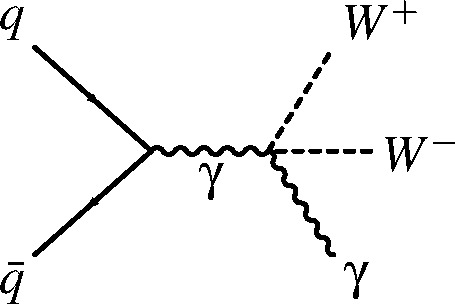
\includegraphics[width=0.35\textwidth]{figs/wwaa.pdf}
%    }
    \hspace{1cm}
%    \subfigure[]{
      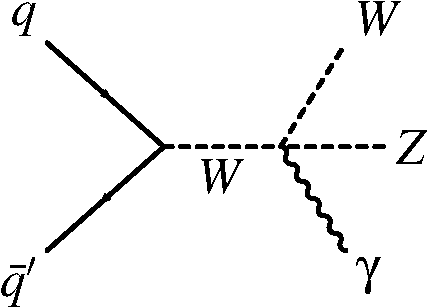
\includegraphics[width=0.35\textwidth]{figs/wwza.pdf}
%    }
}

    \caption{Feynman diagrams that involve a quartic vector boson vertex. Both diagrams are present in the SM.}
    \label{fig:feyndiag}
  \end{center}
\end{figure} 


\begin{eqnarray}\label{lagrangian}
{\cal L}_{\textrm{AQGC}} &=& -\dfrac{e^2}{8} \dfrac{a_0^W}{\Lambda^2} F_{\mu \nu} F^{\mu \nu} W^{+\alpha} W^-_{\alpha} - \dfrac{e^2}{16} 
\dfrac{a_C^W}{\Lambda^2} F_{\mu \nu} F^{\mu \alpha} ( W^{+\nu} W^-_{\alpha} + W^{-\nu} W^+_{\alpha} ) \nonumber \\
& &- e^2 g^2 \dfrac{\kappa_0^{W}}{\Lambda^2} F_{\mu \nu} Z^{\mu \nu} W^{+ \alpha} W^-_{\alpha}- \frac{e^2 g^2}{2} \dfrac{\kappa_C^{W}}{\Lambda^2} F_{\mu \nu} Z^{\mu \alpha} ( W^{+\nu} W^-_{\alpha} + W^{-\nu} W^+_{\alpha} )\nonumber \\ 
& &+ \dfrac{f_{T,0}}{\Lambda^4} Tr[\hat{W}_{\mu \nu} \hat{W}^{\mu \nu}] \times Tr[\hat{W}_{\alpha \beta} \hat{W}^{\alpha \beta}] .
\end{eqnarray}

The dimension 6 parameters $a_0^W/\Lambda^2$ and $a_C^W/\Lambda^2$ are
associated with the WW$\gamma\gamma$ vertex and the
$\kappa_0^W/\Lambda^2$ and $\kappa_C^W/\Lambda^2$ parameters are
associated with the WWZ$\gamma$ vertex. The dimension 8 parameter
$f_{T,0}/\Lambda^4$ contributes to both vertices. The
$a_{0,C}^W/\Lambda^2$ coupling parameters~\cite{Belanger:1999} have
dimension 8 analogues, the $f_{M,i}/\Lambda^4$ coupling parameters. The relationship between the two is as follows:

\begin{center}
\begin{eqnarray}
\dfrac{a_0^W}{\Lambda^2} &= &-\dfrac{4 M_W^2}{g^2} \dfrac{f_{M,0}}{\Lambda^{ 4}} - \dfrac{8 M_W^2}{g^{' 2}} \dfrac{f_{M,2}}{\Lambda^{ 4}}, \nonumber \\ 
\dfrac{a_C^W}{\Lambda^2} &= &\dfrac{4 M_W^2}{g^2} \dfrac{f_{M,1}}{\Lambda^{ 4}} + \dfrac{8 M_W^2}{g^{' 2}} \dfrac{f_{M,3}}{\Lambda^{ 4}},
\label{dim6to8}
\end{eqnarray}
\end{center}
where $g = e/\sin(\theta_W), g^{'} = e/\cos(\theta_W)$, $\theta_W$ is
the Weinberg angle, $e$ is the unit of electric charge, and $\Lambda$
represents the energy scale of possible new physics represented by these operators. 
%The validity of the expressions listed in Eq.~\eqref{dim6to8} are
%checked using numerical simulations, as shown in Figure~\ref{fig:dim6dim8trans}. 
The expressions listed in Eq.~\eqref{dim6to8} are used to translate 
the AQGC limits obtained for $a_{0,C}^W/\Lambda^2$, into limits on $f_{M,i}/\Lambda^4$.

%% \begin{figure}[htb]
%% \begin{center}
%%    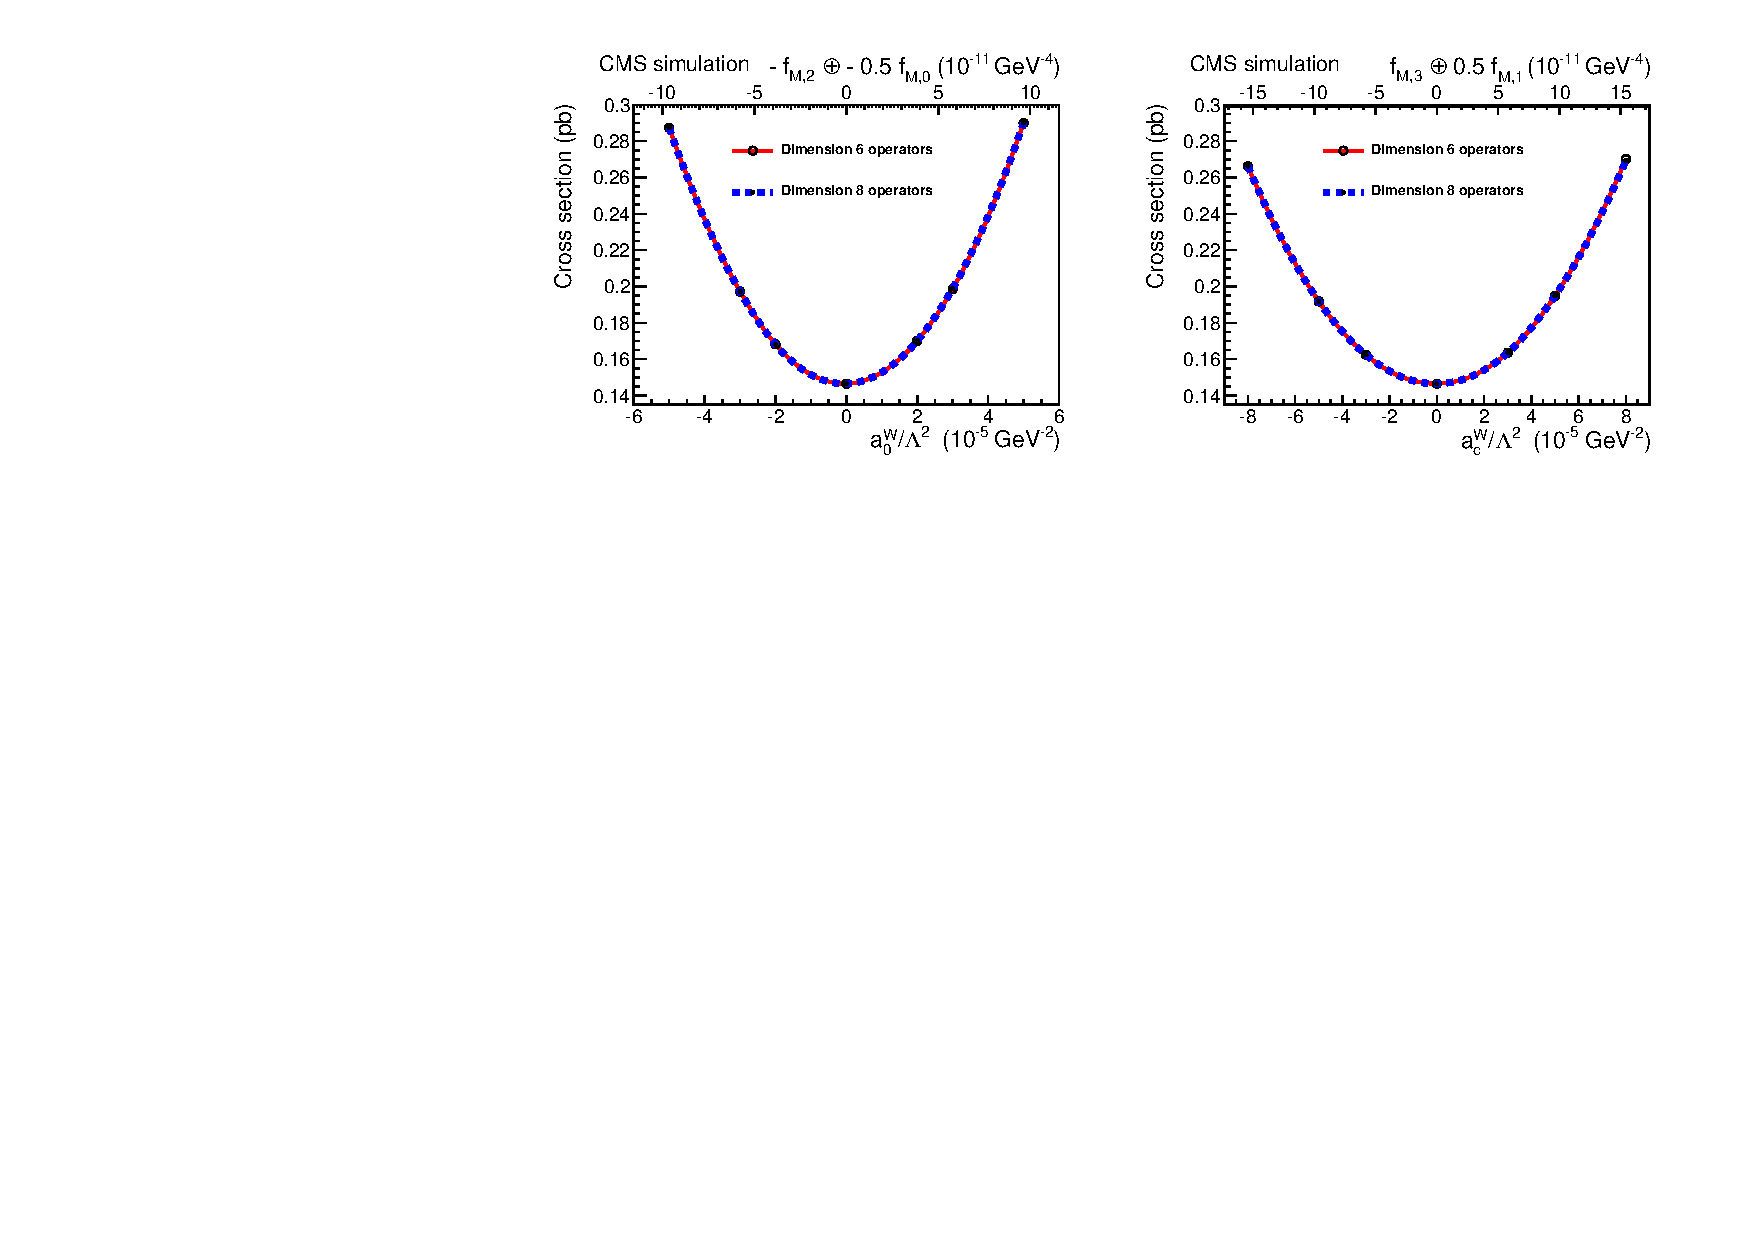
\includegraphics[width=.9\textwidth]{figs/comp628.pdf}
%% \caption{Predictions of the cross section as a function of the dimension 8 parameters $f_{M,i}$ and dimension 6 parameters $a_{0}^W$ and $a_{C}^W$.}
%% \label{fig:dim6dim8trans}
%% \end{center}
%% \end{figure}

Any nonzero value of the AQGCs will lead to tree-level unitarity
violation at sufficiently high energy. Therefore we calculated the
unitarity bounds \cite{Chapon:2009,AQGC:2001} for each AQGC parameter
as a function of $\Lambda_{ff}$ and $\hat{s}$ and substituted in a
dipole form factor $\alpha\rightarrow\frac{\alpha}{(1 +
\hat{s}/\Lambda_{ff}^2)^2}$, where $\alpha$ is an AQGC parameter,
$\Lambda_{ff}$ is the form factor scale and $\sqrt{\hat{s}}$ is the
center-of-mass energy of the interacting partons.  Illustration of the
unitarity bound and the expected limits are shown in Figure
\ref{fig:unitarity} for $a_{0}^{W}/\Lambda^{2}$,
$a_{C}^{W}/\Lambda^{2}$, and $f_{T,0}/\Lambda^{4}$, as a function of
$\Lambda_{ff}$.  The typical value for $\sqrt{\hat{s}}$ is 2~TeV for
values of the AQGC parameters close to the expected
limits~(Section \ref{sec:limits_pT}).

Figure~\ref{fig:unitarity} indicates that the effective field theory
terms directly violate unitarity at parameter values close to the
expected limits, and that the unitarity condition cannot be generally
satisfied for any scale $\Lambda_{ff}$ by the addition of such a form
factor. However, unitarity conserving new physics with a structure
more complex than that represented by a dipole form factor is
possible, making this search directly sensitive to new physics.  Since
the structure of such new physics is not known \textit{a priori}, the
choice is made to set limits without using form factors.  
%At 14 TeV, with larger data sets, these searches will also be directly sensitive
%to new physics that can be represented by an effective field theory.


\begin{figure}[hb]
  \begin{center}
    \subfigure[]{
    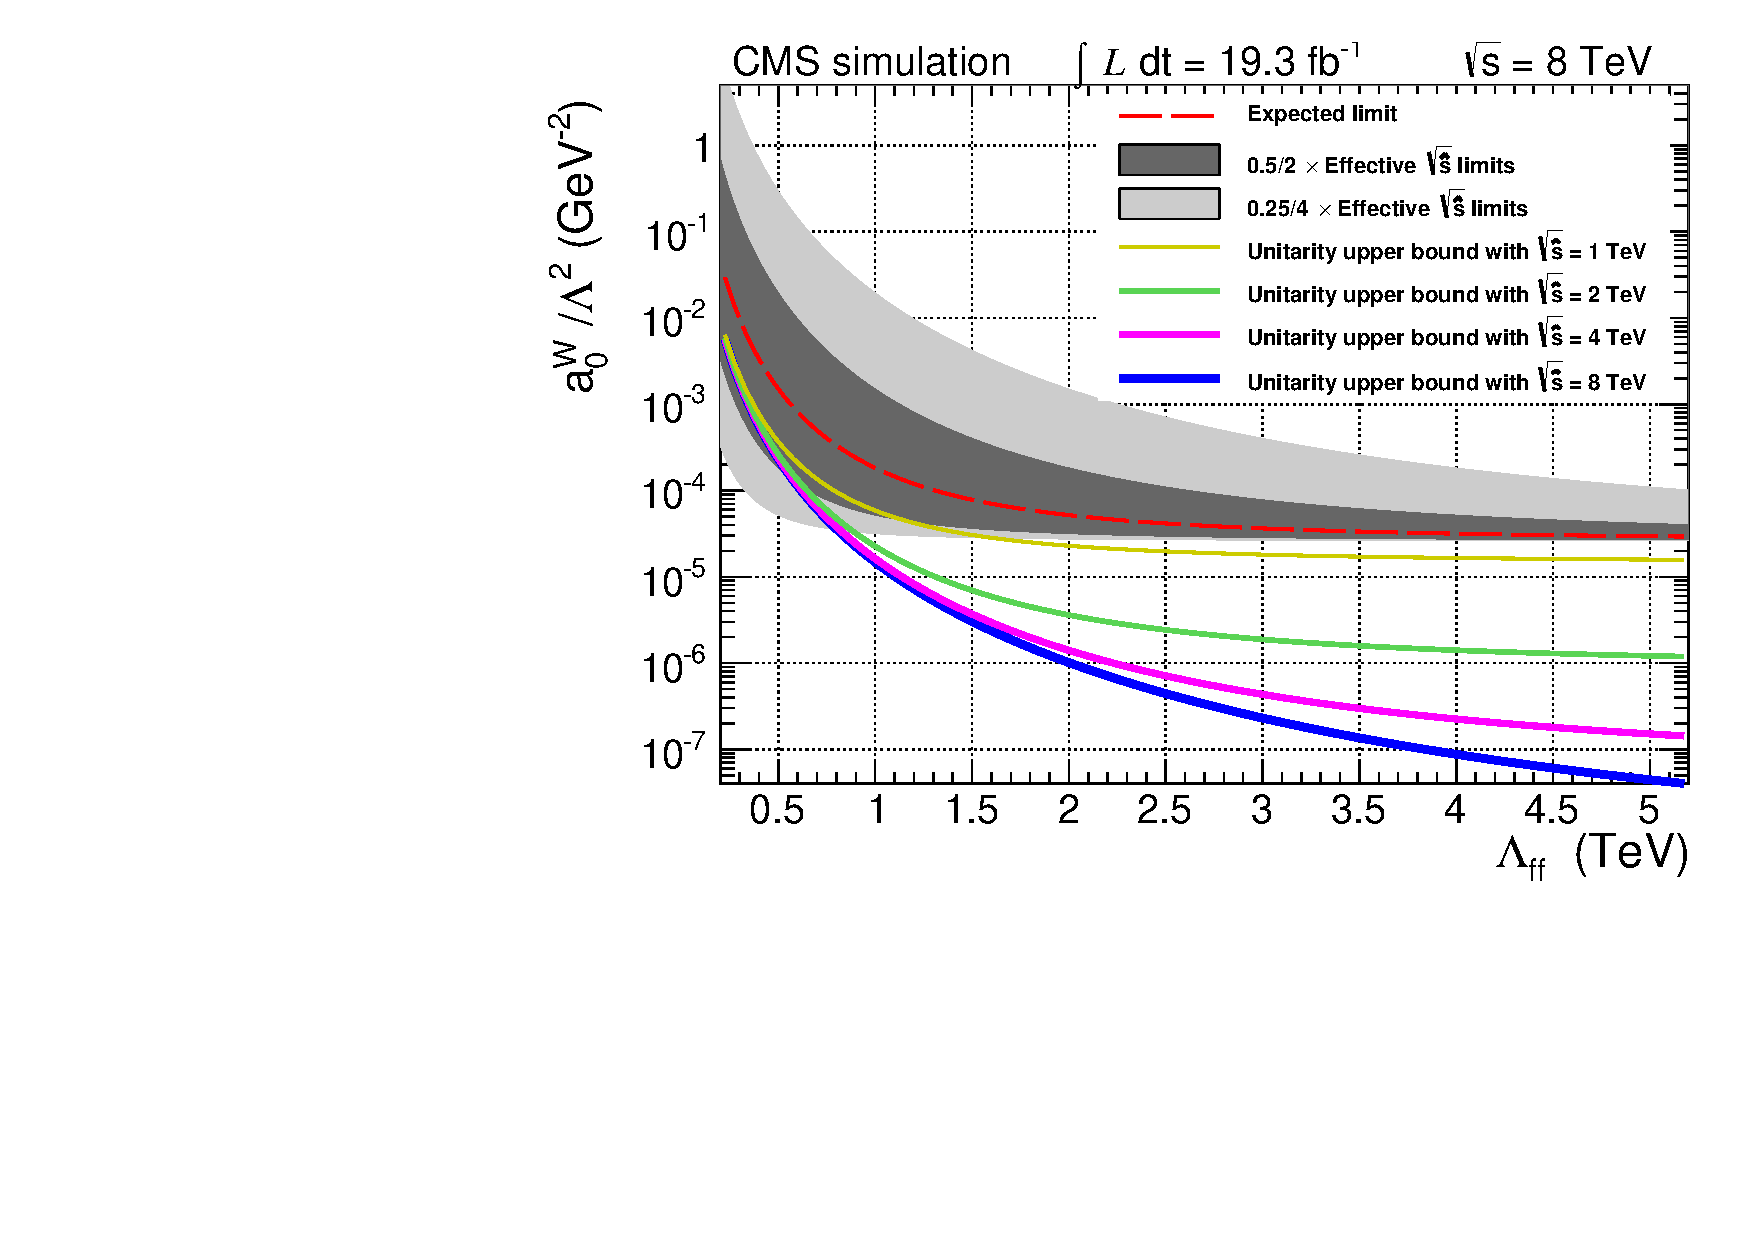
\includegraphics[width=0.51\textwidth]{figs/prounitarity_a0w.pdf}
  }
    \subfigure[]{
    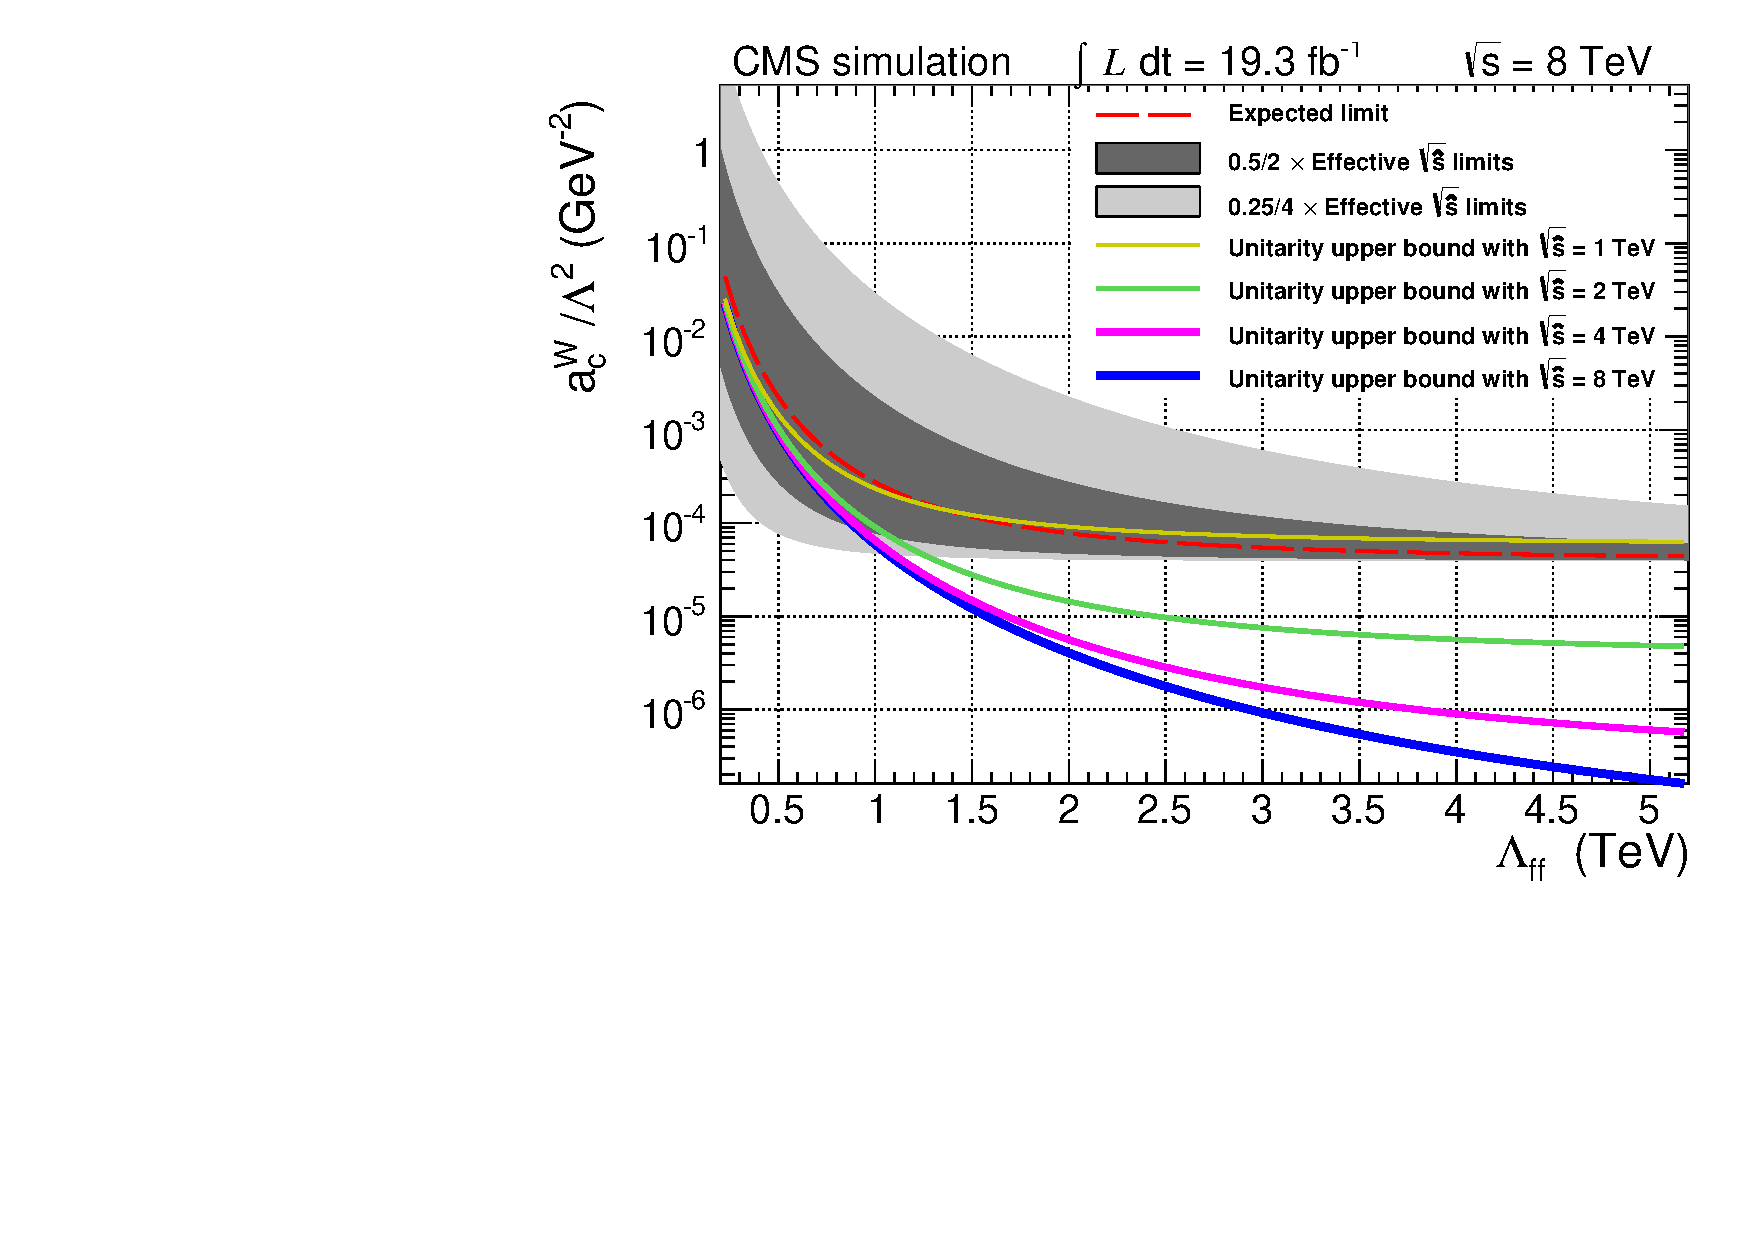
\includegraphics[width=0.51\textwidth]{figs/prounitarity_acw.pdf}
  }\\
  \subfigure[]{
    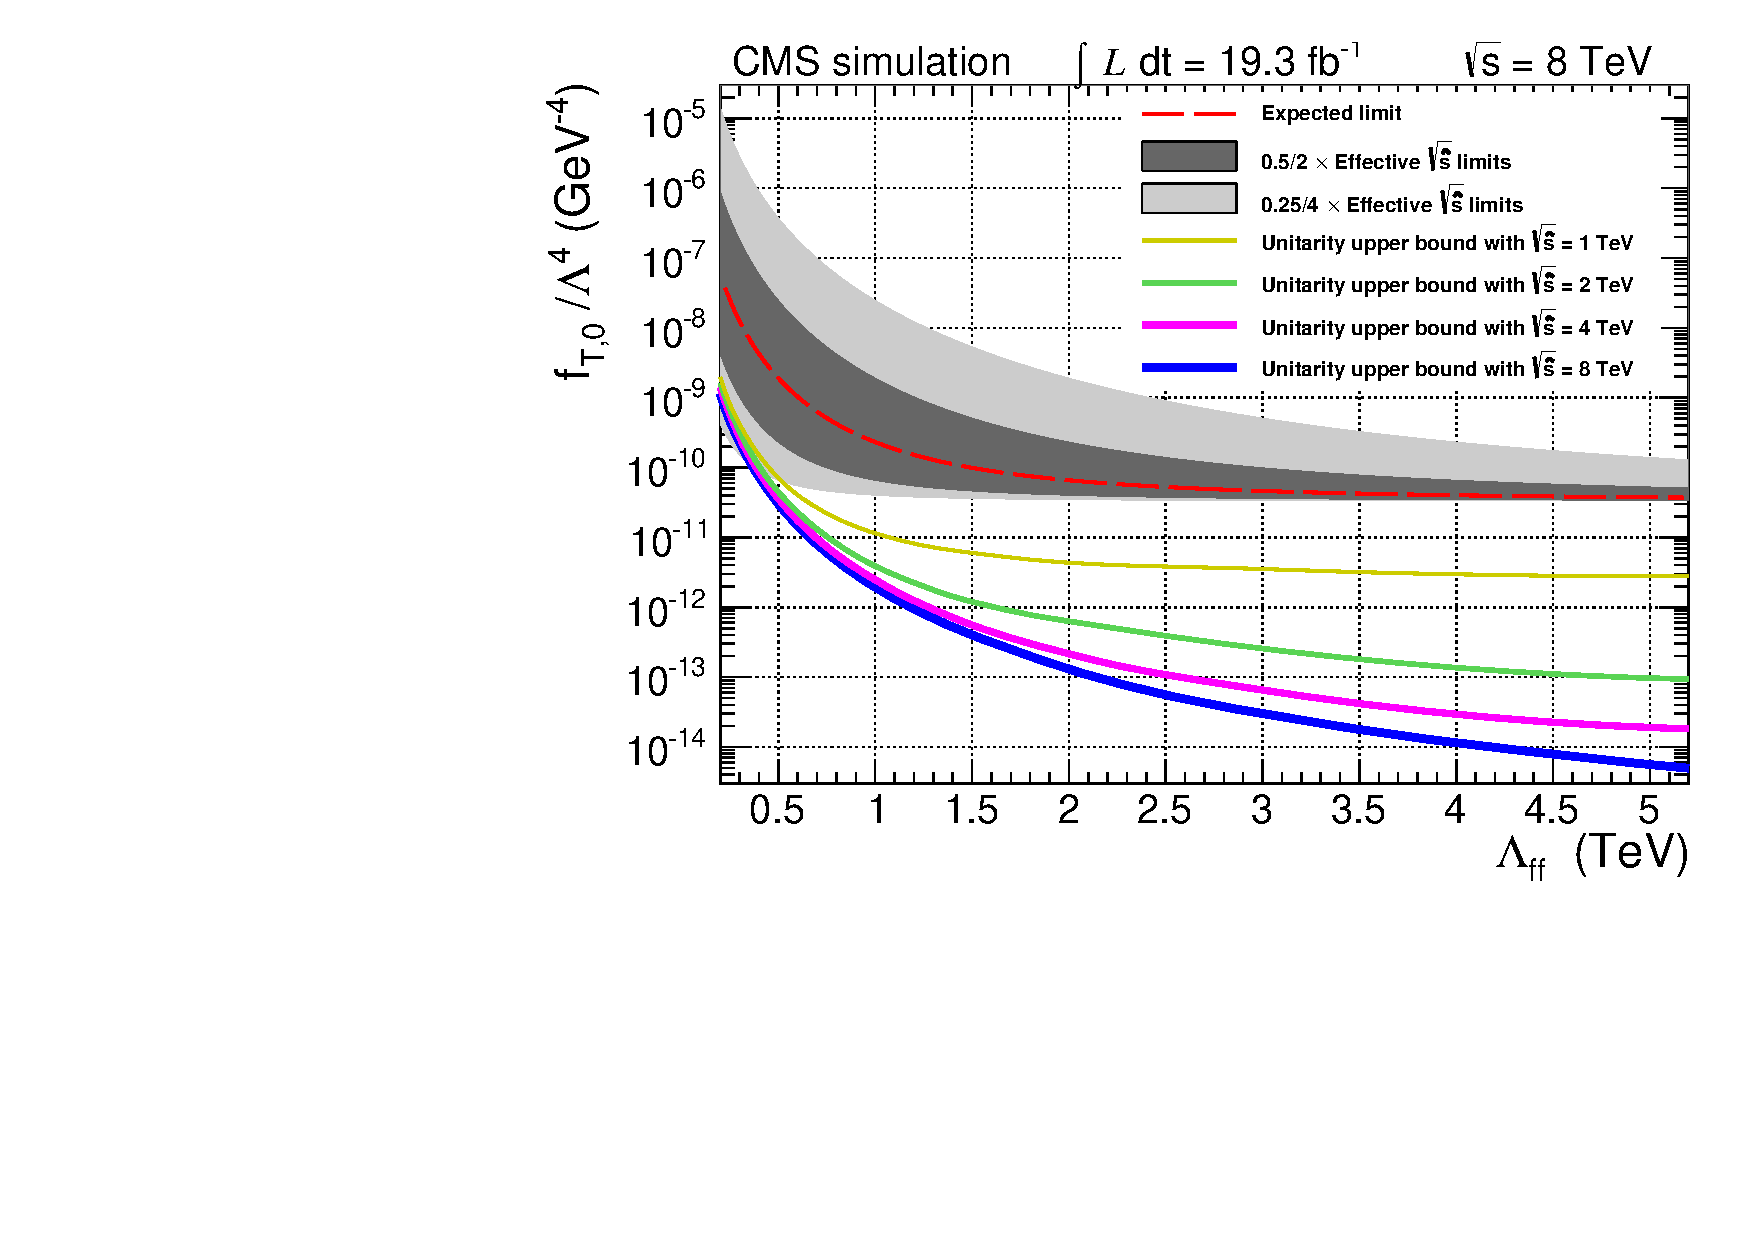
\includegraphics[width=0.51\textwidth]{figs/prounitarity_fT0.pdf}
  }
  \subfigure[]{
    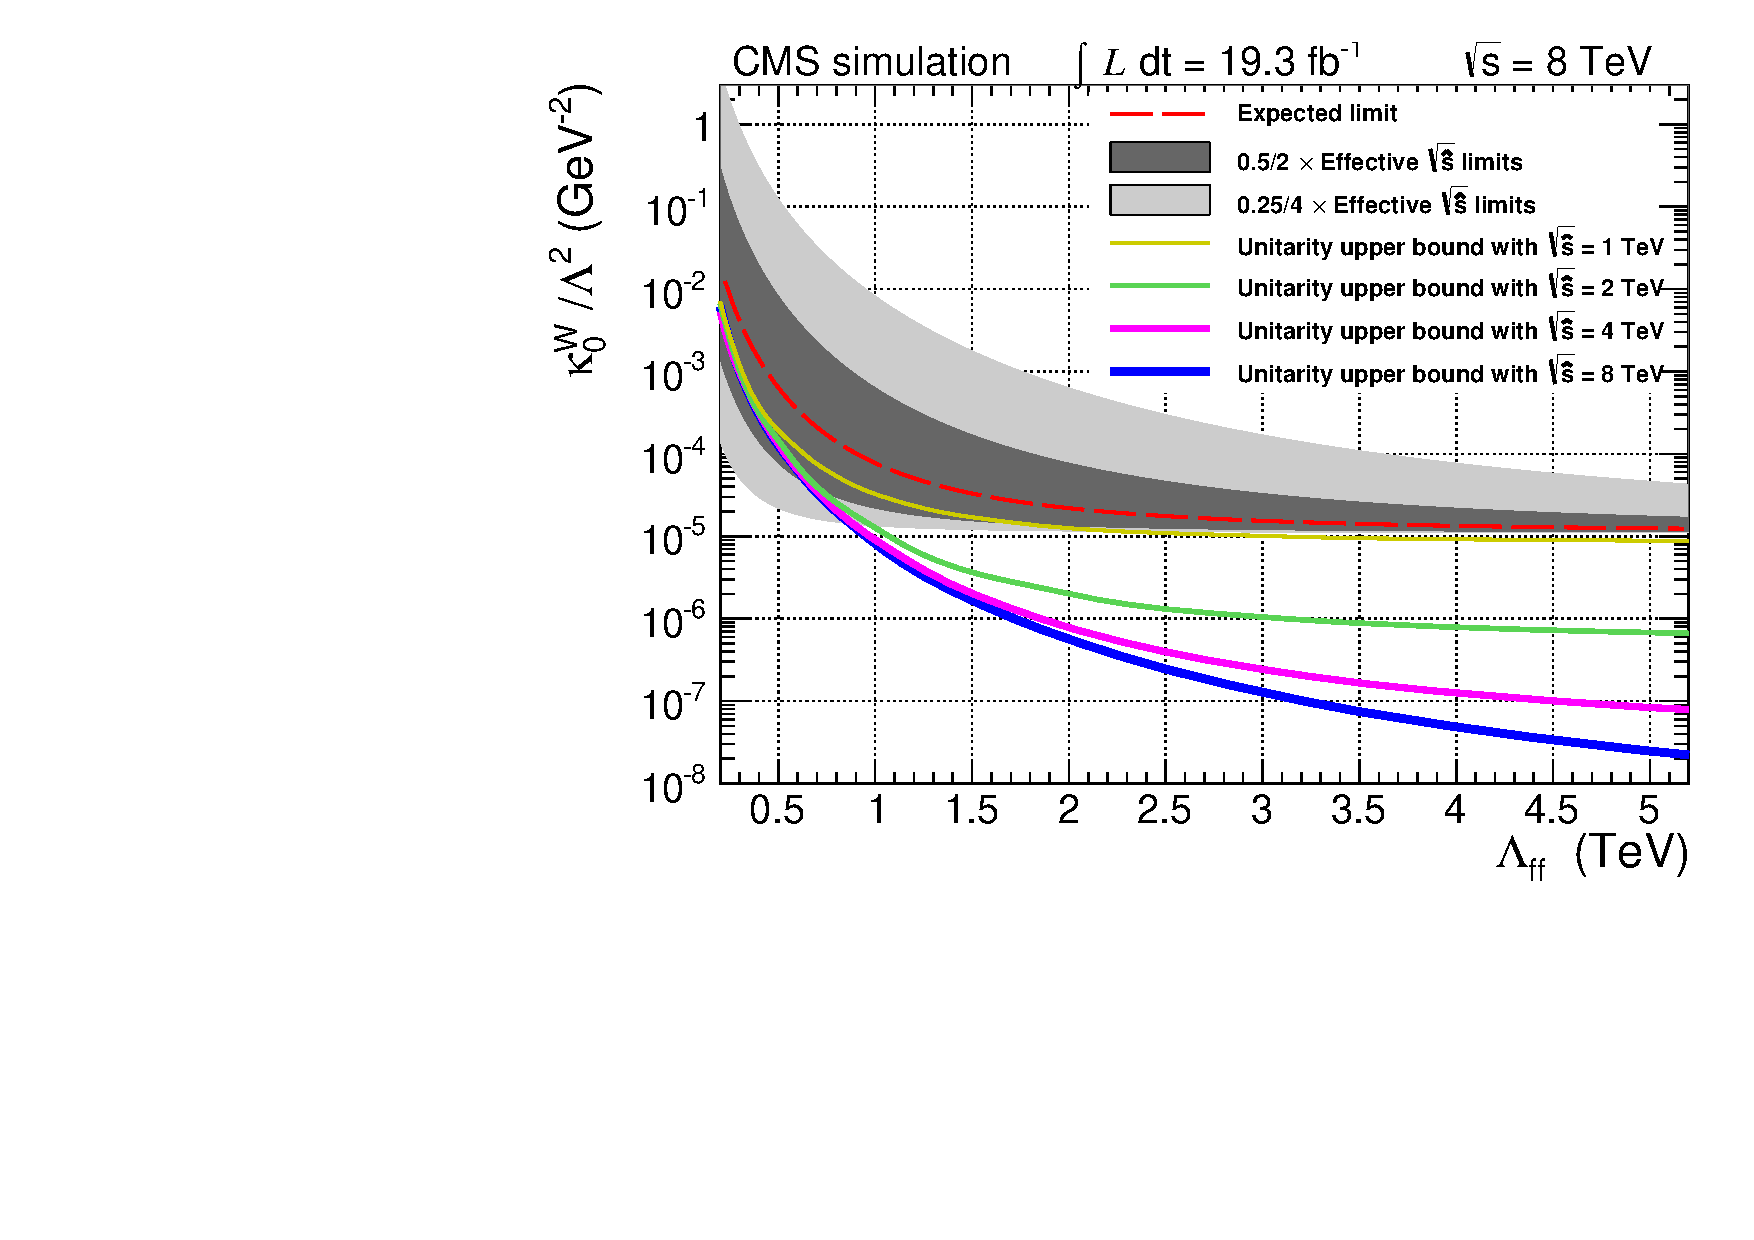
\includegraphics[width=0.51\textwidth]{figs/prounitarity_k0W.pdf}
  } \\
  \subfigure[]{
    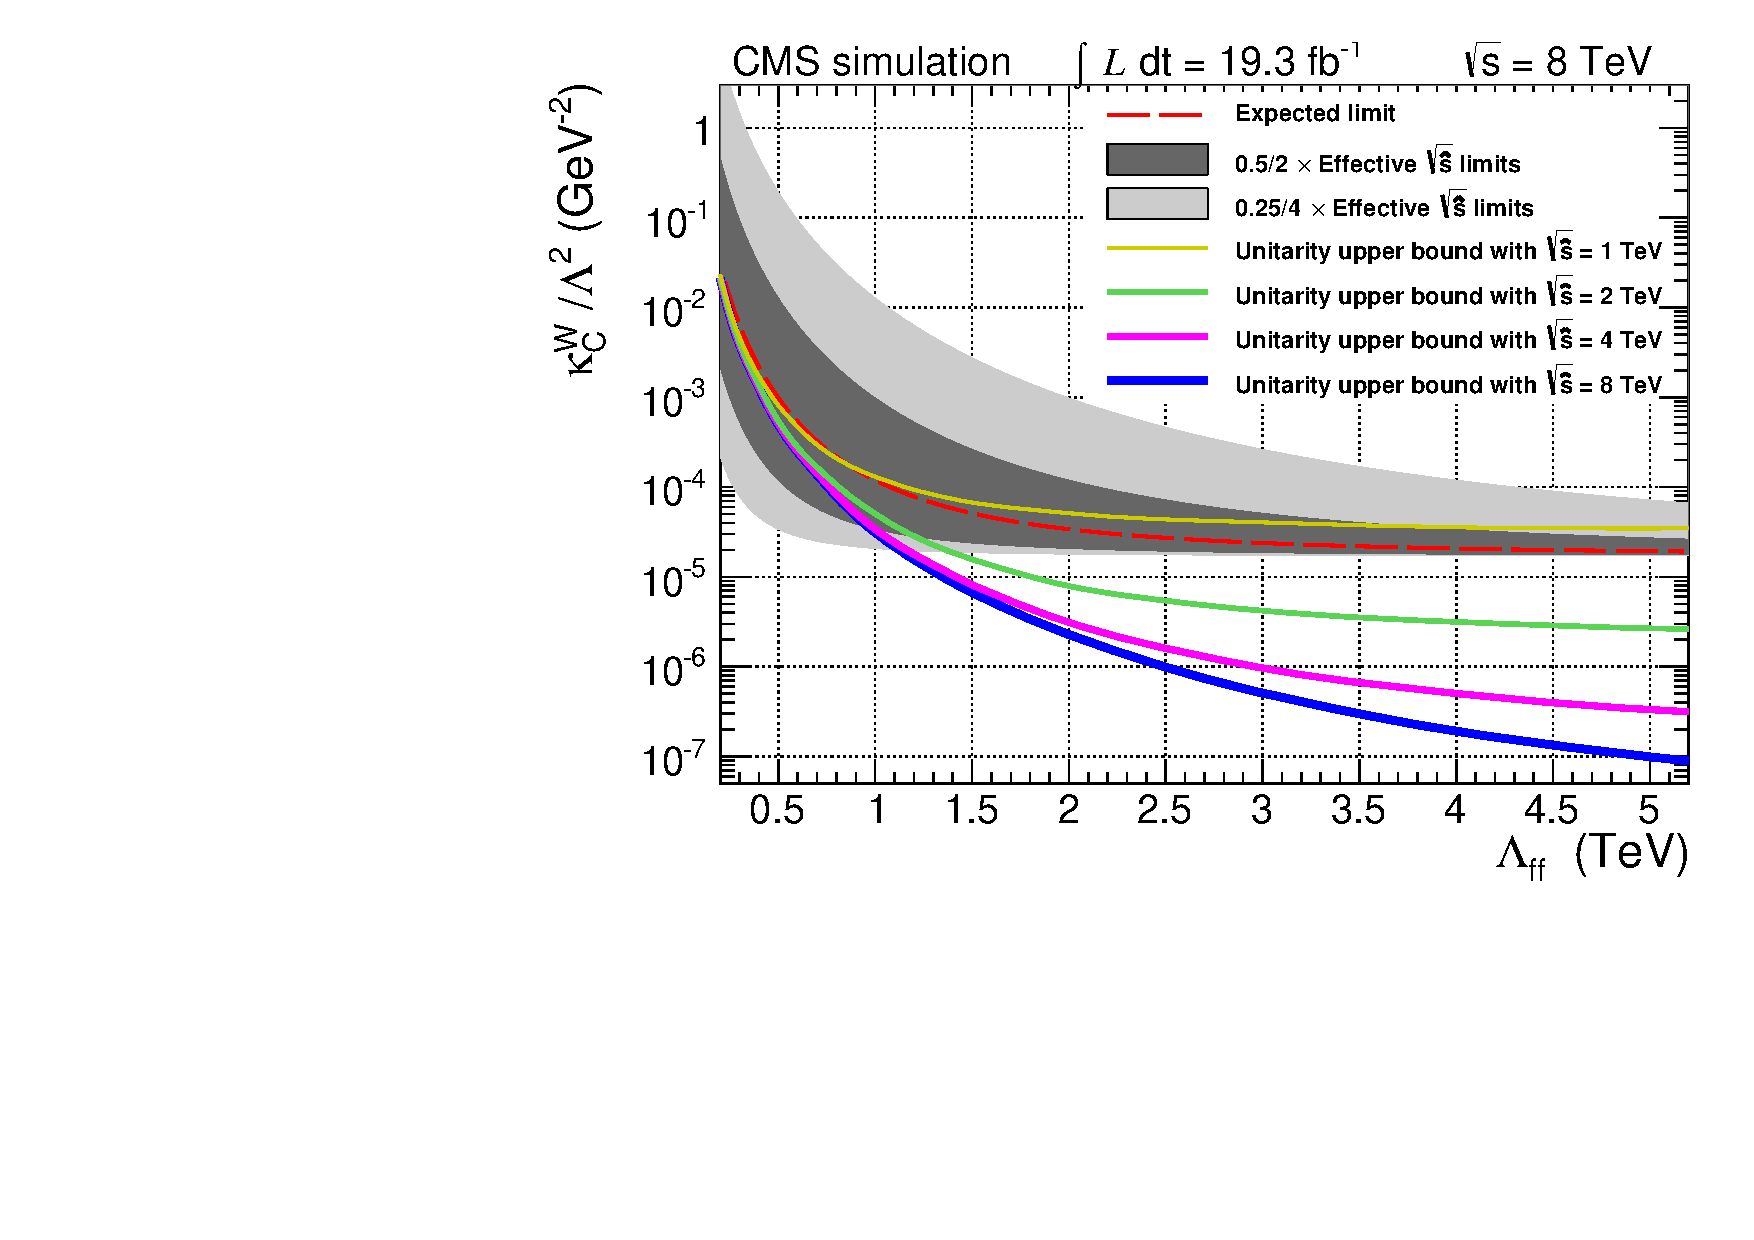
\includegraphics[width=0.51\textwidth]{figs/prounitarity_kCW.pdf}
  }
    \caption{ Unitarity bound as a function of the dipole form factor
scale $\Lambda_{ff}$ for (a) $a_{0}^{W}/\Lambda^{2}$, (b)
$a_{C}^{W}/\Lambda^{2}$, (c) $f_{T,0}/\Lambda^{4}$, (d)
$\kappa_{0}^{W}/\Lambda^{2}$, and (e) $\kappa_{C}^{W}/\Lambda^{2}$.
The dashed red lines represent the expected limits of this analysis,
and the gray bands represent regions around the expected limits with
$\hat{s}$ varied by a factor of 2 or 4. The colored curves represent
the unitarity bounds for fixed values of $\hat{s}$, above which
unitarity is violated.}
    \label{fig:unitarity}
  \end{center} \end{figure}

